\documentclass[tikz,border=12pt]{standalone}
\usepackage[T1]{fontenc}
\usepackage{lmodern,amsmath,amssymb}
\usetikzlibrary{arrows.meta,positioning,calc}
\definecolor{ink}{HTML}{183444}
\definecolor{blue}{HTML}{1B6780}
\definecolor{amber}{HTML}{AD601A}
\begin{document}
\hyphenpenalty=10000\exhyphenpenalty=10000
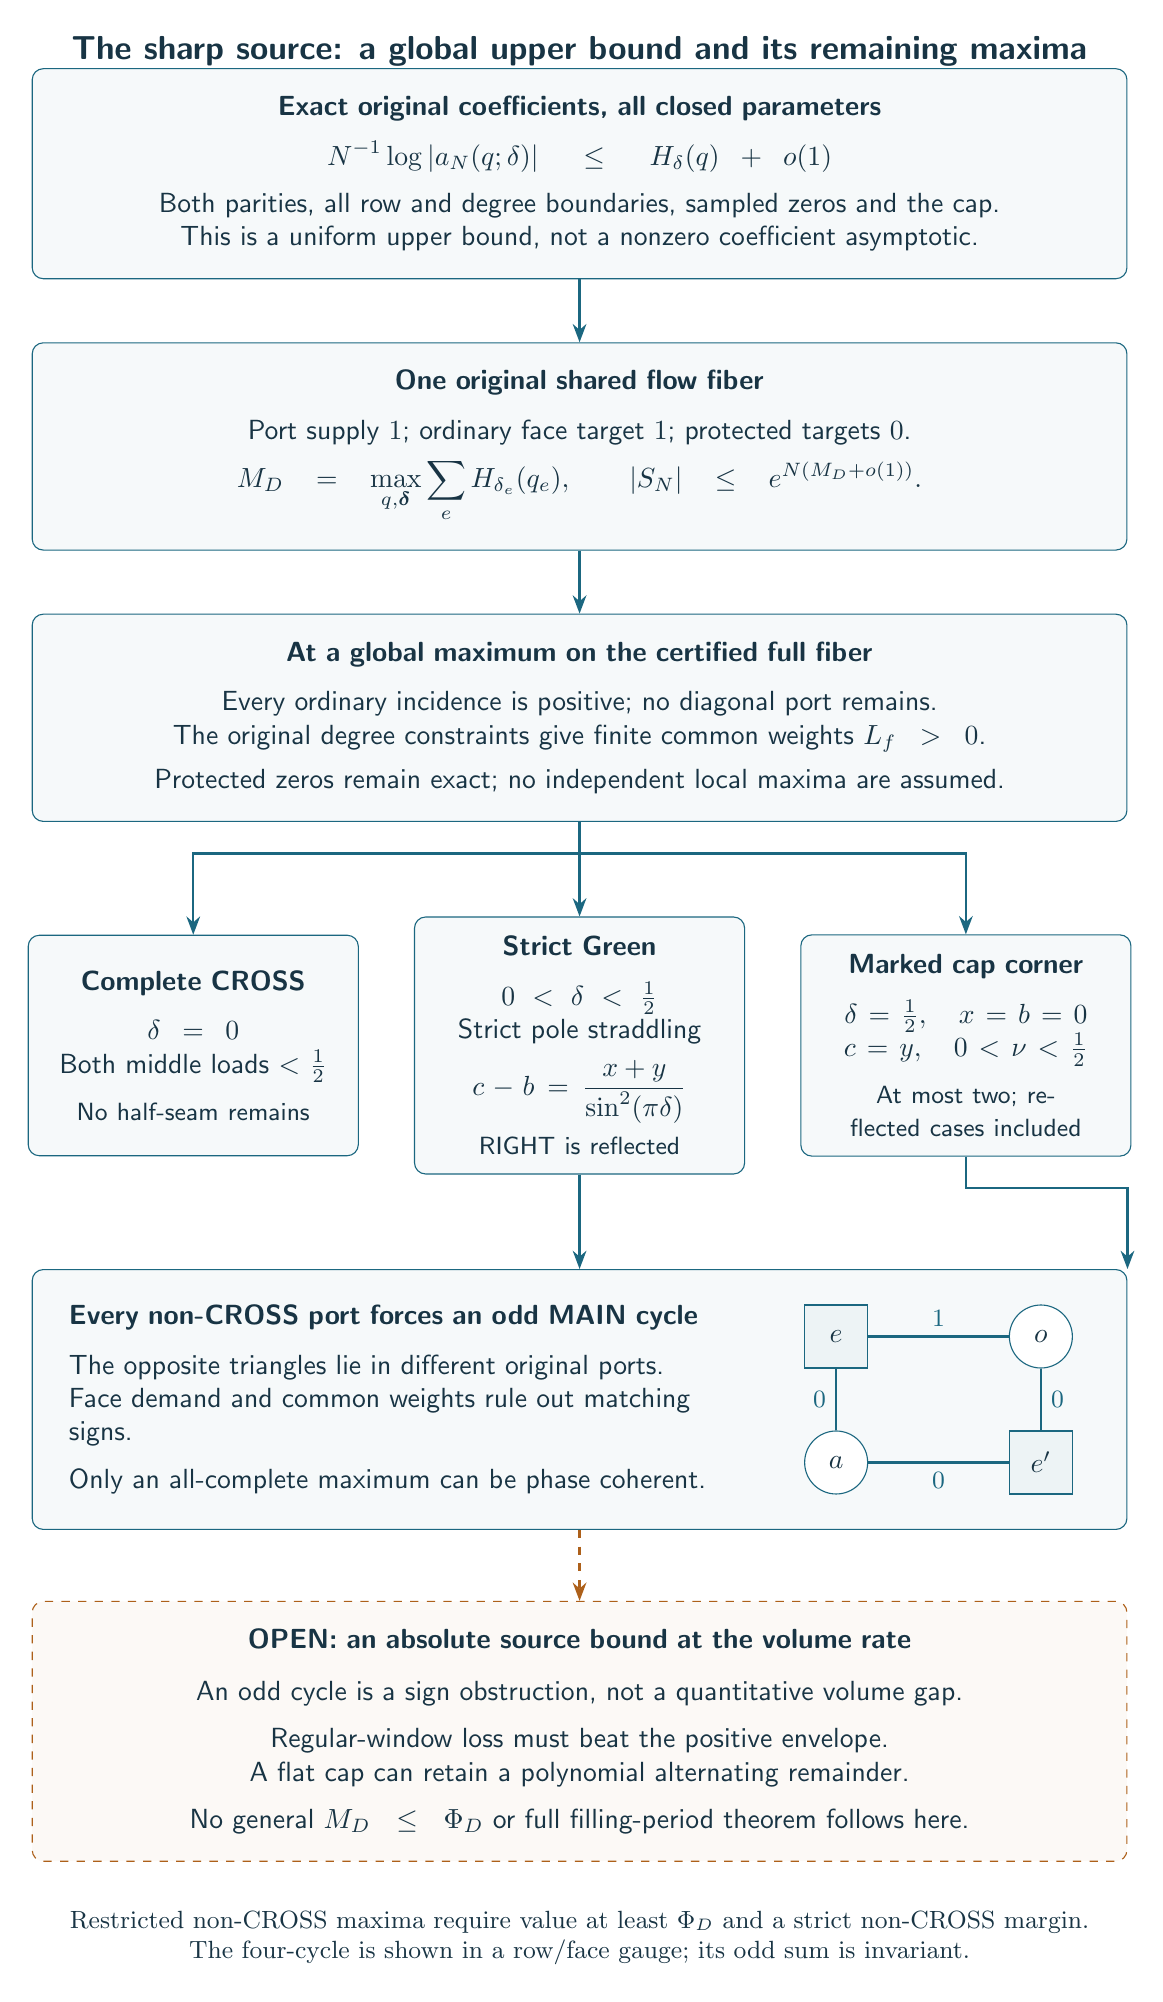
\begin{tikzpicture}[font=\sffamily,text=ink,>=Stealth,
 panel/.style={draw=blue,fill=blue!4,rounded corners,align=center,
 text width=13.2cm,inner sep=10pt},
 branch/.style={panel,text width=37mm,minimum height=28mm,inner sep=7pt},
 pending/.style={panel,draw=amber,fill=amber!4,dashed},
 face/.style={circle,draw=blue,fill=white,minimum size=8mm},
 port/.style={rectangle,draw=blue,fill=blue!8,minimum size=8mm}]
\node[font=\sffamily\large\bfseries] at (0,0)
 {The sharp source: a global upper bound and its remaining maxima};
\node[panel] (source) at (0,-1.55)
 {\textbf{Exact original coefficients, all closed parameters}\\[6pt]
 $\displaystyle N^{-1}\log|a_N(q;\delta)|\le H_\delta(q)+o(1)$\\[5pt]
 Both parities, all row and degree boundaries, sampled zeros and the cap.\\
 This is a uniform upper bound, not a nonzero coefficient asymptotic.};
\node[panel,below=8mm of source] (fiber)
 {\textbf{One original shared flow fiber}\\[6pt]
 Port supply $1$; ordinary face target $1$; protected targets $0$.\\[4pt]
 $\displaystyle M_D=\max_{q,\boldsymbol\delta}\sum_eH_{\delta_e}(q_e),
 \qquad |S_N|\le e^{N(M_D+o(1))}.$};
\draw[->,thick,blue] (source)--(fiber);
\node[panel,below=8mm of fiber] (regular)
 {\textbf{At a global maximum on the certified full fiber}\\[6pt]
 Every ordinary incidence is positive; no diagonal port remains.\\
 The original degree constraints give finite common weights $L_f>0$.\\[4pt]
 Protected zeros remain exact; no independent local maxima are assumed.};
\draw[->,thick,blue] (fiber)--(regular);

\node[branch,below=12mm of regular.south] (green)
 {\textbf{Strict Green}\\[6pt]
 $0<\delta<\tfrac12$\\
 Strict pole straddling\\[5pt]
 $\displaystyle c-b=\frac{x+y}{\sin^2(\pi\delta)}$\\[4pt]
 \small RIGHT is reflected};
\node[branch,left=7mm of green] (cross)
 {\textbf{Complete CROSS}\\[6pt]
 $\delta=0$\\
 Both middle loads $<\tfrac12$\\[5pt]
 \small No half-seam remains};
\node[branch,right=7mm of green] (cap)
 {\textbf{Marked cap corner}\\[6pt]
 $\delta=\tfrac12,\quad x=b=0$\\
 $c=y,\quad 0<\nu<\tfrac12$\\[5pt]
 \small At most two; reflected cases included};
\draw[->,thick,blue] (regular.south)--(green.north);
\draw[->,thick,blue] (regular.south) -- ++(0,-.4) -| (cross.north);
\draw[->,thick,blue] (regular.south) -- ++(0,-.4) -| (cap.north);

\node[panel,below=12mm of green.south,minimum height=33mm] (cycle) {};
\node[align=left,text width=8.2cm,anchor=west] at ($(cycle.west)+(.35,0)$)
 {\textbf{Every non-CROSS port forces an odd MAIN cycle}\\[6pt]
 The opposite triangles lie in different original ports.\\
 Face demand and common weights rule out matching signs.\\[5pt]
 Only an all-complete maximum can be phase coherent.};
\node[port] (e) at ($(cycle.east)+(-3.7,.8)$) {$e$};
\node[face] (o) at ($(cycle.east)+(-1.1,.8)$) {$o$};
\node[port] (ep) at ($(cycle.east)+(-1.1,-.8)$) {$e'$};
\node[face] (a) at ($(cycle.east)+(-3.7,-.8)$) {$a$};
\draw[thick,blue] (e)--node[above,font=\small] {$1$}(o);
\draw[thick,blue] (o)--node[right,font=\small] {$0$}(ep);
\draw[thick,blue] (ep)--node[below,font=\small] {$0$}(a);
\draw[thick,blue] (a)--node[left,font=\small] {$0$}(e);
\draw[->,thick,blue] (green.south)--(cycle.north);
\draw[->,thick,blue] (cap.south)--++(0,-.4)-|(cycle.north east);

\node[pending,below=9mm of cycle] (open)
 {\textbf{OPEN: an absolute source bound at the volume rate}\\[7pt]
 An odd cycle is a sign obstruction, not a quantitative volume gap.\\[5pt]
 Regular-window loss must beat the positive envelope.\\
 A flat cap can retain a polynomial alternating remainder.\\[5pt]
 No general $M_D\le\Phi_D$ or full filling-period theorem follows here.};
\draw[->,thick,amber,dashed] (cycle)--(open);
\node[align=center,font=\small,text width=13.2cm,below=5mm of open]
 {Restricted non-CROSS maxima require value at least $\Phi_D$ and a strict
 non-CROSS margin.\\The four-cycle is shown in a row/face gauge; its odd sum is invariant.};
\end{tikzpicture}
\end{document}
